\documentclass{llncs}

\usepackage{amsmath}
\usepackage{url}
\usepackage{makeidx} % allows for index generation
\usepackage{multirow}
\usepackage{graphicx}
\usepackage{float}
\usepackage{titling}
\usepackage{array}
\usepackage{filecontents}
\usepackage{subcaption}
\captionsetup{compatibility=false}

\setlength{\pdfpageheight}{\paperheight}
\setlength{\pdfpagewidth}{\paperwidth}

% constants
\def\cvc{CVC4}
\def\us{Z3str3}
\def\fuzzer{StringFuzz}
\def\generator{StringFuzzG}
\def\transformer{StringFuzzX}
\def\smt{SMT-LIB 2.0/2.5}

\def\numSolvers{four}
\def\theSolvers{\us{}, Norn, \cvc{}, and ABC}

\def\problemRepo{https://example.com}
\def\sourceRepo{https://github.com/dblotsky/stringfuzz}

\begin{document}

    % styles
    \pagestyle{headings} % switches on printing of running heads
    \addtocmark{Hamiltonian Mechanics} % additional mark in the TOC

    % title
    \title{
        \fuzzer{}: A Fuzzer for String Solvers
    }
    \titlerunning{\fuzzer{}} % abbreviated title (for running head)

    % authors
    \author{
        Dmitry Blotsky\inst{1}\orcidID{0},
        Federico Mora\inst{1}\orcidID{0},
        Murphy Berzish\inst{1}\orcidID{0},\and
        Ifaz Kabir\inst{1}\orcidID{0},
        Vijay~Ganesh\inst{2}\orcidID{1}
    }
    \authorrunning{Dmitry Blotsky et al.}

    % institutions
    \institute{
        University of Waterloo, Waterloo ON, Canada,\\
        \email{dblotsky@uwaterloo.ca}
    }

    \maketitle

    \begin{abstract}

    In this paper we present StringFuzz: an SMT-LIB problem fuzzer and generator for string solvers. With it we analyse \numSolvers{} mature string solvers: \theSolvers{}. We use it to craft inputs that elicit poor performance in Z3str3 and CVC4, and provide analyses of the causes of the performance degradations. Our experimental data suggest that there are classes of problems that will always be hard for Z3str3 and easy for CVC4, and vice versa, due to the limitations of the core algorithms implemented by those solvers. We also present several minor bugs in Z3str3 that were exposed by StringFuzz. Finally, we provide a rich repository of problems in SMT-LIB format, generated both by StringFuzz and by hand, to encourage other solver authors to likewise improve their solvers.

\end{abstract}

    \section{Introduction}

In recent years, many algorithms for solving string constraints have
been developed and implemented in SMT solvers such as Norn~\cite{norn},
CVC4~\cite{cvc4}, and Z3 (e.g., Z3str2~\cite{z3str2} and Z3str3~\cite{z3str3}).
To validate and benchmark these solvers, their developers have relied on
hand-crafted input suites~\cite{cvc4-tests,z3str3-tests,z3str2-tests} or
real-world examples from a limited set of industrial
applications~\cite{kaluza,kausler}. These test suites have helped
developers identify implementation defects and develop more
sophisticated solving heuristics. Unfortunately, as solvers grow,
these benchmarks remain stagnant, leaving increasing functionality untested.
As such, there is an acute need for a more robust, inexpensive, and automatic way
of generating benchmarks to test
the correctness and performance of SMT solvers.

Fuzzing has been used to test all kinds of software
including SAT solvers~\cite{fuzzsat}. Inspired by the utility of fuzzers,
we introduce \fuzzer{} and describe its value
as an exploratory testing tool. We demonstrate its efficacy
by presenting limitations it helped discover in
leading string solvers. To the best of our knowledge, \fuzzer{} is the
only tool aimed at automatic generation of string constraints. \fuzzer{} can
be used to mutate or transform existing benchmarks, as well as
randomly generate structured instances. These instances can be scaled with
respect to a variety of parameters, e.g., length of string constants,
depth of concatenations (concats) and regular expressions (regexes),
number of variables, number of length constraints, and many more.

\subsubsection{Contributions}

\begin{enumerate}
    \item \textbf{The \fuzzer{} tool}:
        In Sect.~\ref{sec:fuzzer}, we describe a modular fuzzer that can
        transform and generate \smtfull{} string and regex
        instances.\footnote{We assume basic
        familiarity with string solvers and their input
        language.} Scaling inputs (e.g., long string constants,
        deep concatenations) are particularly useful in identifying asymptotic
        behaviors in solvers, and \fuzzer{} has many options to generate them.
        We briefly document \fuzzer{}'s components and modular architecture.
        We provide example use cases to demonstrate its utility as an
        exploratory solver testing tool.

    \item \textbf{A repository of \smtfull{} instances}:
        We present a repository of \smtfull{} string and regex instance suites
        that we generated using \fuzzer{} in Sect.~\ref{sec:suites}. This
        repository consists of two categories: one with new
        instances generated by \fuzzer{} (\texttt{generated}); and another with
        transformed instances generated from a small suite of industrial
        benchmarks (\texttt{transformed}).

    \item \textbf{Experimental Results and Analysis}:
        We compare the performance of \theSolvers{} on the
        \fuzzer{} suites \theSuites{} in Sect.~\ref{sec:data}. We
        highlight these suites because they make some solvers perform poorly,
        but not others. We analyze our
        experimental results, and pinpoint algorithmic limitations
        in \us{} that cause poor performance.
\end{enumerate}

    \section{\fuzzer{}}
\label{sec:fuzzer}

\subsubsection{Implementation and Architecture}

\fuzzer{} is implemented as a Python package, and comes with several
executables to generate, transform, and analyze \smtfull{} string and regex
instances. Its components are implemented as \unix{} ``filters'' to enable easy
integration with other tools (including themselves). For example, the
outputs of generators can be piped into transformers, and transformers
can be chained to produce a stream of tuned inputs to a
solver. \fuzzer{} is composed of the following tools:
\begin{description}
    \item[\generator{}] \hfill \\
    This tool generates \smt{} instances. It supports several generators and
    options that specify its output. Details can be found in
    Table~\ref{tbl:generators}.
    \item[\transformer{}] \hfill \\
    This tool transforms \smt{}
    instances. It supports several transformers and options that specify
    its output and input, which are explained in
    Table~\ref{tbl:transformers}. Note that transformers
    \textit{Translate} and \textit{Reverse} also preserve
    satisfiability under certain conditions~\cite{ifaz}.
    \item[\texttt{stringstats}] \hfill \\
    This tool takes an \smt{}
    instance as input and outputs its properties: the number of
    variables/literals, the max/median syntactic depth of expressions, the
    max/median literal length, etc.
\end{description}
We organized \fuzzer{} to be easily extended. As evidence of our success we note
that while the whole project
contains \linesInFuzzer{} lines of code, it takes an average of
\linesPerX{} lines of code to create a transformer. \fuzzer{} can either be
installed from source, or from the Python PIP package
repository.\footnote{The link to the source code will be added after double-blind review.}

\begin{table}[t]
    \caption{\fuzzer{} built-in (a) generators and (b) transformers.}
    \begin{subtable}{1\textwidth}
        \centering
        \caption{\generator{} built-in generators.}
        \label{tbl:generators}
        \begin{tabular}{ l l }
            \toprule
            \textbf{Name}
            & \textbf{Generates instances that have ...} \\
            \midrule
            \textit{Concats}
            & Long concats and optional random extracts. \\
            \textit{Lengths}
            & Many variables (and their concats) with length constraints. \\
            \textit{Overlaps}
            & An expression of the form A.X = X.B. \\
            \textit{Equality}
            & An equality among concats, each with variables or constants. \\
            \textit{Regex}
            & Regexes of varying complexity. \\
            \textit{Random-Text}
            & Random, likely syntactically \textit{in}valid text. \\
            \textit{Random-AST}
            & Random, but semantically \textit{valid} text. \\
            \bottomrule
        \end{tabular}
    \end{subtable}
    \begin{subtable}{1\textwidth}
        \centering
        \caption{\transformer{} built-in transformers.}
        \label{tbl:transformers}
        \begin{tabular}{l l}
            \toprule
            \textbf{Name}
            & \textbf{The transformer ...} \\
            \midrule
            \textit{Fuzz}
            & Replaces literals and operators with similar ones.\\
            \textit{Graft}
            & Randomly swaps non-leaf nodes with leaf nodes.\\
            \textit{Multiply}\footnote{Satisfiable inputs
            will produce satisfiable outputs (see Appendix for proof).}
            & Multiplies integers and repeats strings by N.\\
            \textit{Nop}
            & Does nothing (can translate between \smtfull{}).\\
            \textit{Reverse}\footnote{Input and output
            instances will be equisatisfiable (see Appendix for proof).}
            & Reverses all string literals and concat arguments.\\
            \textit{Rotate}
            & Rotates compatible nodes in syntax tree.\\
            \textit{Translate}\footnotemark[4]
            & Permutes the alphabet.\\
            \textit{Unprintable}
            & Replaces characters in literals with unprintable ones.\\
            \bottomrule
        \end{tabular}
    \end{subtable}
\end{table}

\subsubsection{Regex Generating Capabilities}
\fuzzer{} can generate
and transform instances with regular expression constraints. For example, 
\texttt{stringfuzzg regex} invokes the regex
generator and produces an instance of the form:
\begin{align*}
    & \texttt{(assert (str.in.re X}\; R_0\; \texttt{))} \\
    & \texttt{(assert (str.in.re X}\; R_n\; \texttt{))}* \\
    & \texttt{(assert (<= Min (str.len X)))}? \\
    & \texttt{(assert (<= (str.len X)) Max)}?
\end{align*}

where $R_i \in RegEx$, and $Min, Max \in Int$. More simply, the
instance is a set of one or more regex constraints on a single
variable, with optional maximum and minimum length constraints. The
regex constraints $R$ are each of the form:
\begin{align*}
    & \texttt{(re.++}\; T_0\; \texttt{(re.++}\; T_1\;
    \texttt{...}\; \texttt{(re.++}\; T_{n-1}\; T_n\; \texttt{))}
\end{align*}

and each $T_i$ is a recursive term of the form:
\begin{align*}
    & \texttt{(re.*}\; T_{i_j}\; \texttt{) | (re.+}\; T_{i_j}\;
    \texttt{) | (re.union}\; T_{i_{j_1}}\; T_{i_{j_2}}\; \texttt{)}
\end{align*}

where $j$ is the specified depth of recursion. Terms at depth 0 are
regex constants. Informally, this form describes a concatenation of
regex terms, where each term is a random nested regex operator (chosen from
regex Kleene star, repetition, and union), up to a specified depth,
terminating in a regex literal. Below are three example regex instances
(separated by spaces) of depth 2 produced by this scheme:
\begin{align*}
    & ((\texttt{a}|\texttt{b})|(\texttt{cc})+)\quad\quad
    ((\texttt{ddd})*)+\quad\quad ((\texttt{ee})+|(\texttt{fff})*)
\end{align*}

\subsubsection{Equisatisfiable String Transformations}
\fuzzer{} can also transform problem instances.
This is done by manipulating parsed syntax trees.
By default most of the built-in transformers
only guarantee well-formedness, however,
some can even guarantee equisatisfiability. Table~\ref{tbl:transformers}
lists the built-in transformers and notes these guarantees.

\subsubsection{Example Use Case}
In Sect.~\ref{sec:suites} we use \fuzzer{} to generate benchmark suites in a batch mode.
We can also use \fuzzer{} for on-line exploratory debugging.
For example, the script below repeatedly feeds random \fuzzer{}
instances to \cvc{} until the solver produces an error:
{\scriptsize\begin{verbatim}
while stringfuzzg -r random-ast -m \
    | tee instance.smt25 | cvc4 --lang smt2.5 --tlimit=5000 --strings-exp; do
    sleep 0
done\end{verbatim}}

    \section{Problem Suites}

    Along with this paper we present several suites of ready-made problems produced by StringFuzz. These suites can be found on \problemRepo{}.

    \subsection{\fuzzer{}-Generated}

        This suite contains the following problem sets:

        \begin{itemize}
            \item Lengths
            \item Lengths-Concats
            \item Concats
            \item Concats-Extracts
            \item Overlaps
            \item Regex
            \item Many-Regexes
            \item Regex-Deep
            \item Regex-Pair
            \item Regex-Lengths
            \item Random??
        \end{itemize}

        Most of these problem sets either have a dedicated generator in \generator{}, or are variations of one. While it is likely that some of the pre-made suites will be immediately useful in analysing a solver, we also found that mass randomisation was helpful in finding some bugs, and we encourage this pattern as well. \generator{} is designed to be used in an exploratory fashion, and the following usage has helped us in our own experiments:

\begin{verbatim}
while true; do stringfuzzg --random regex | z3str3 -in; done
\end{verbatim}

    \subsection{\fuzzer{}-Transformed}

        This suite contains the following problem sets:

        \begin{itemize}
            \item Amazon??
            \item Regex??
        \end{itemize}

        Most of these problem sets were generated by using one root problem and transforming it with \transformer{} into many similar problems.

    \subsection{Unit Tests}

        This suite covers corner cases of solver behaviour. We have used the instances in this suite to find bugs in \us{}.

    \subsection{Results}

        This section describes the bugs in \us{} that were discovered (and subsequently fixed) by testing it with the \fuzzer{} problem suites.

        \begin{enumerate}
            \item length lookup using eqc root
            \item length-testing bug
        \end{enumerate}
    \section{Experimental Results and Analysis}
\label{sec:data}

We generated several problem suites with \fuzzer{} that made one
solver perform poorly, but not others. These suites are
\theSuites{}. Figure~\ref{fig:cvc-hard} shows the suites that were
uniquely difficult for \cvc{}. Figure~\ref{fig:z3str3-hard} shows the
suites that were uniquely difficult for \us{}. All experiments were
run in series, with a timeout of 15 seconds, on the same computer running
Ubuntu Linux 16.04. The computer had 32GB of RAM and an
Intel\textregistered{} Core\texttrademark{} i7-6700 CPU with clock speed
of 3.40GHz.

\begin{figure}[h]
    \begin{subfigure}{.5\textwidth}
        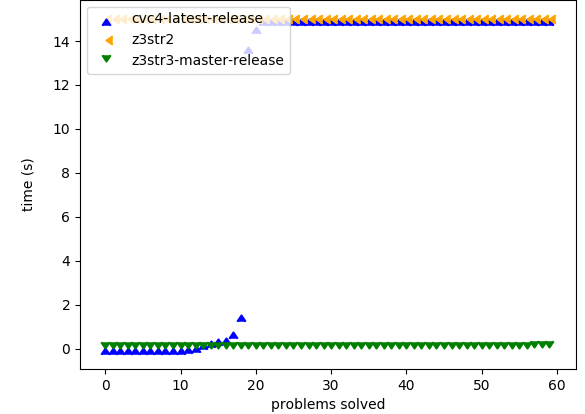
\includegraphics[width=\textwidth]{data/graphs/concats-extracts-small.png}
        \caption{Performance on concats-extracts-small}
        \label{fig:concats-extracts-small}
    \end{subfigure}
    \begin{subfigure}{.5\textwidth}
        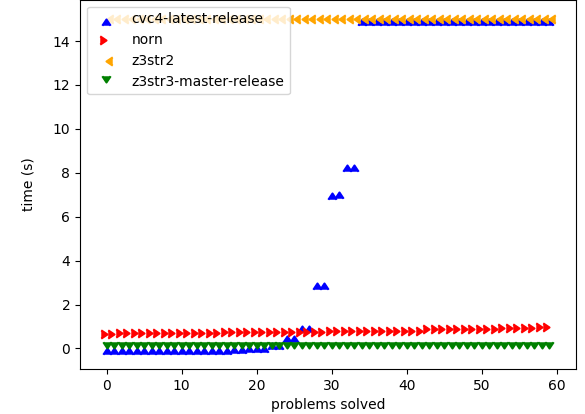
\includegraphics[width=\textwidth]{data/graphs/different-prefix.png}
        \caption{Performance on different-prefix}
        \label{fig:different-prefix}
    \end{subfigure}
    \caption{Problems hard for \cvc{}}
    \label{fig:cvc-hard}

    \begin{subfigure}{.5\textwidth}
        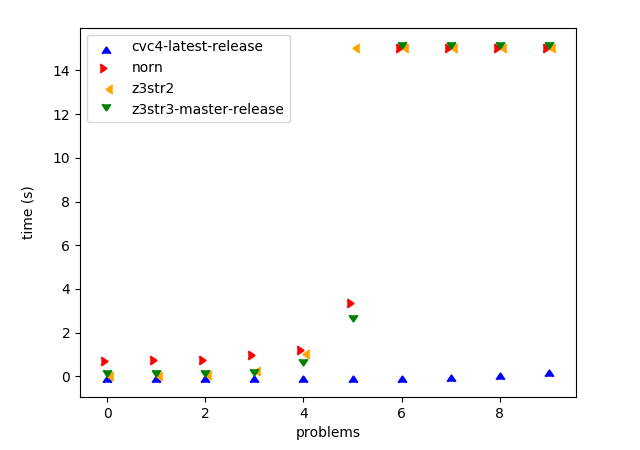
\includegraphics[width=\textwidth]{data/graphs/concats-balanced.png}
        \label{fig:concats-balanced}
        \caption{Performance on concats-balanced}
    \end{subfigure}
    \begin{subfigure}{.5\textwidth}
        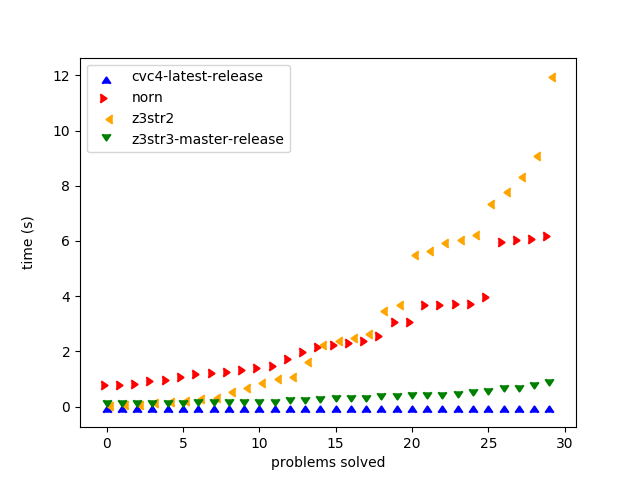
\includegraphics[width=\textwidth]{data/graphs/concats-small.png}
        \label{fig:concats-small}
        \caption{Performance on concats-small}
    \end{subfigure}
    \caption{Problems hard for \us{}}
    \label{fig:z3str3-hard}
\end{figure}

\subsubsection{Usefulness to \us{}: A Case Study}

We found a number of performance-related issues and opportunities for
new heuristics in \us{} thanks to \fuzzer{}. For example, the
instances in the \textit{concats-big} suite generated by \fuzzer{}
helped us discover a missing heuristic. In particular, \us{} didn't
make full use of the solving context (e.g. some terms are empty
strings) to simplify the concatenations of a long list of string terms
before trying to reason about the equivalences among subterms. \us{}
therefore introduced a large number of unnecessary intermediate
variables and propagations. As an immediate consequence of
testing \us{} on \textit{concats-big} benchmarks, we were able to
identify the factors common to these instances and rapidly formulate a
hypothesis as to why they were performing poorly.

    \section{\us{} Recommendation}

    This section outlines a change for \us{}, which we believe will improve its performance on the Eager-Hard problem set and similar problems. We recommend a partial order treatment of equivalence class comparisons. First, we describe a partial order of equivalence classes. Then, we use it in equivalence class comparisons and more closely approximate equality between them.

    % TODO:
    % - definition of partial order
    % - definition of current class relation
    % - definition of class relation under partial order

    \section{Related Work}

Naturally, many solver developers author their own test suites to
validate their solvers~\cite{cvc4-tests,z3str3-tests,z3str2-tests}. In
addition, several popular problem suites are publicly available for
solver validation, such as the Kaluza~\cite{kaluza} and
Kausler~\cite{kausler} suites. There are likewise several fuzzers and
problem generators currently available, but none of them can generate
or transform string and regex problems. For example, the
FuzzSMT~\cite{fuzzsmt} tool generates \smt{} problems with bit-vectors
and arrays, but does not support strings or regexes. The
SMTpp~\cite{smtpp} tool pre-processes and simplifies problems, but
does not generate new ones or fuzz existing ones.


    \bibliographystyle{abbrv}
    \bibliography{paper}

    % \appendix
    % \section{Appendix}

\end{document}
